\documentclass{bioinfo}
\copyrightyear{2015} \pubyear{2015}

\access{Advance Access Publication Date: Day Month Year}
\appnotes{Manuscript Category}
\usepackage{blindtext}

\begin{document}
\firstpage{1}


\subtitle{Subject Section}

\title[Title]{Title}
\author[Sample \textit{et~al}.]{Author\,$^{\text{\sfb 1,}*}$, Author 2\,$^{\text{\sfb 2}}$}
\address{$^{\text{\sf 1}}$Address, \\
$^{\text{\sf 2}}$Address 2}

\corresp{$^\ast$To whom correspondence should be addressed.}

\history{Received on XXXXX; revised on XXXXX; accepted on XXXXX}

\editor{Associate Editor: XXXXXXX}

\abstract{\blindtext}

\maketitle

\section{Introduction}

\blindtext

\section{Section 1}

\blindtext

\begin{figure}[!tpb]
\centerline{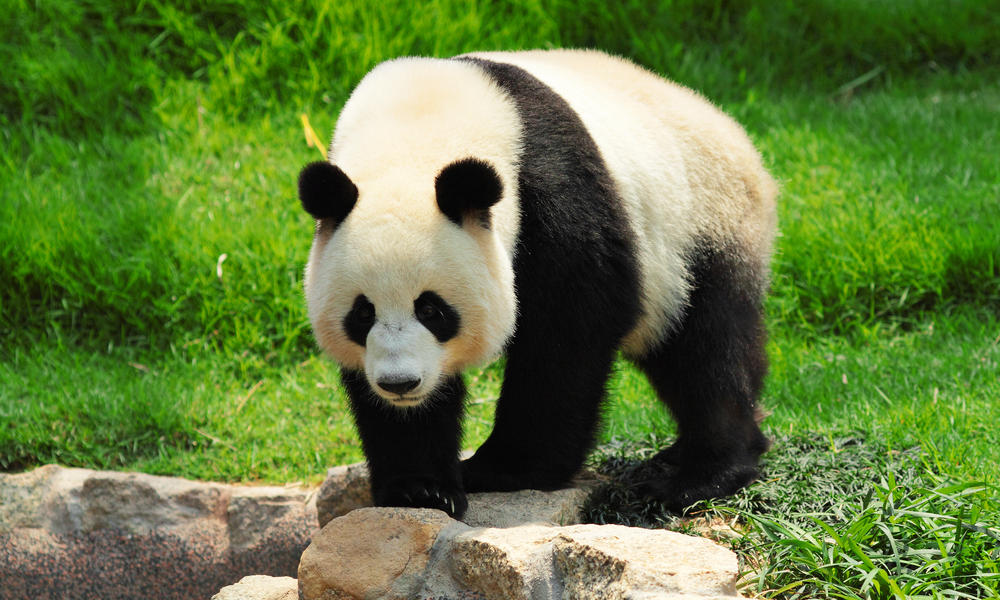
\includegraphics[width=\columnwidth]{panda.jpg}}
\caption{Caption text. 
\label{panda}}
\end{figure}

\begin{figure}[ht!]
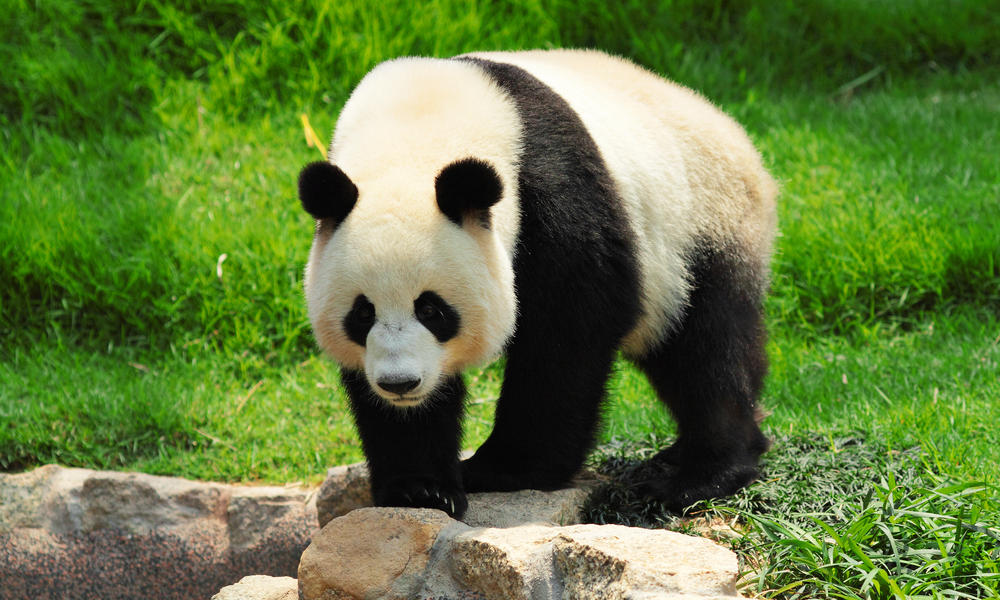
\includegraphics[scale=0.5]{panda.jpg}
\caption{Fix this one.}
\label{panda2}
\end{figure}

\blindtext
%\section{Section 2}
\blindtext
\blindtext
\blindtext
\blindtext
\blindtext
\section{Section 2}
\blindtext
\begin{figure}[h!tb]
\centerline{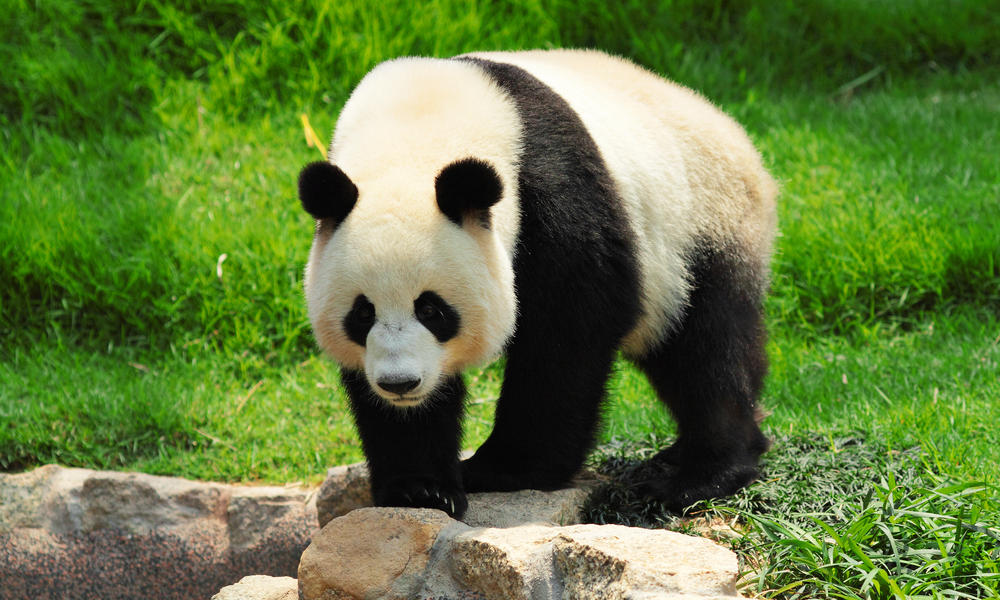
\includegraphics[width=\columnwidth]{panda.jpg}}
\caption{Panda.
\label{panda3}}
\end{figure}


\end{document}
